\documentclass[a4paper]{article}
\usepackage{german}
\usepackage{fontenc}
\usepackage[ansinew]{inputenc}
\usepackage{epsfig}
\usepackage{graphicx}
%\usepackage{sistyle}
\usepackage{listings}
\usepackage{amsmath}

\topmargin-1.0cm
\textheight23.0cm
\textwidth14cm
\addtolength{\oddsidemargin}{-0.9cm}

\begin{document}

%\begin{titlepage}
\begin{center}



\vspace{7cm}


\textbf\huge{{Die Konvektion des Mondes}}\\
\vspace{2cm}
\large{Geodynamik planetarer K�rper}\\
\vspace{1cm}
WiSe 2011/2012
\vspace{2cm}
Doreen Kasper\\
\vspace{1cm}
\today

\end{center}

\textbf{damit der Abstand zwischen kopfzeile und text auf den Seiten, die nicht mit einer �berschrift beginnen, nicht so klein ist: --> Seitenbeginn mit newpage manuell festlegen und dann als erstes ein bigskip oder doppelbackslash einf�gen}

\end{titlepage}
\begin{titlepage}
\begin{center}
\vspace{7cm}
\huge{\textbf{�bungsaufgaben zur Potenzialtheorie}}\\
\vspace{2cm}
\large{WiSe 2012/2013}\\
\vspace{2cm}
Janina Kammann\\ Marius kriegerowski\\ Moritz Nieschlag\\ Doreen Kasper\\
\vspace{1cm}
\today
\end{center}
\end{titlepage}


\thispagestyle{empty} 
\tableofcontents
\newpage
\thispagestyle{empty}
\listoffigures
\thispagestyle{empty} 

\newpage
\setcounter{page}{1}
\section{Aufgabenteil 1}
Im Rahmen der Masterveranstaltung \textit{GP-M-POTTHEO} wurden uns die mathematisch-physikalischen Grundlagen der Potentialtheorie vermittelt, welche nun in den folgenden �bungen an ausgew�hlten geophysikalischen Beispielen veranschaulicht werden. Die hierf�r verwendeten Programme sowie graphischen Darstellungen wurden mittels der Software Matlab erstellt und sind dem anschlie�enden Anhang dieser Arbeit zu entnehmen. Die von uns verwendeten Gleichungen zur Aufgabenbearbeitung basieren auf dem Vorlesungeskript oder in der Vorlesung bereitgestellter Literatur.\\
\\

Im ersten Aufgabenteil des �bungsblattes sollen drei S�tze Legendre Polynome als Funktion der geographischen L�nge und Breite berechnet und programmiert werden. Die jeweiligen Polynome unterscheiden sich durch verschiedene Ordnungen n und Grade m, wobei f�r diese folgende Bedingung gilt: $m \le n$.\\
Die in den anschlie�enden Darstellungen berechneten Polynome definieren sich aus folgender Beziehung:

\begin{equation}
(A_{n,m}cosm\Phi + B_{n,m}sinm\Phi)*P^{m}_{n}(\theta)
\end{equation}

Laut Aufgabenstellung gilt f�r die Koeffizienten der Zusammenhang: $A_{n,m}=B_{n,m}=1$
Da die Legendre-Polynome auf der Verwendung beliebig orthogonaler Funktionen basieren haben wir f�r die Normalisierung der zonalen Kugelfunktionen eine Schmidt-Normalisierung mittels der Matlabfunktion \textit{'sch'} durchgef�hrt, sodass aus der Basis des aufgespannten Vektorraums eine Orthnormalbasis konstruiert wird. Durch die Normalisierung wird des Weiteren eine Wichtung der Koeffizienten in einem Intervall von $[-1,1]$ vorgenommen.\\
Die nachfolgenden Darstellungen zeigen die Ergebnisse der programmierten Legendre-Polynome. Der entsprechend dokumentierte Programmcode ist dem Anhang A zu entnehmen.\\
\\
Die erste Graphik veranschaulicht eine zonale Darstellung der Legendre-Polynome. In diesem Fall ist die Ordnung des Polynoms stets durch m=0 definiert und der Grad des Polynoms variierbar (hier n=9). Da Polynom $P^{0}_{9}$ definiert sich �ber 9 Nullstellen und ist unabh�ngig von den L�ngengraden ($\theta$) (da m=0). Verschiedene Beispiele zeigen, dass durch Erh�hung der Koeffizienten m und n die beschriebenen Gebiete der Funktion kleiner 'gef�chert' sind. 
Die zweite Abbildung f�r $P^{6}_{6}$ ist sektoriell, das hei�t der Grad des Polynoms entspricht seiner Ordnung sodass gilt: m=n=6. In diesem Fall ist das Polynom unabh�ngig von dem Breitengrad und durch 12 Nullstellen definiert. Die dritte Graphik veranschaulicht die allgemeine Kugelfl�chenfunktion $P^{3}_{9}$; eine tesserale Darstellung der unterschiedlichen Koeffizienten. 
 
\begin{figure}[h!]
	\center
	\includegraphics[scale=0.7]{zonal.eps}
	\caption{Legendre-Polynom $P^{0}_{9}$ - zonal}
\end{figure}

\begin{figure}[h!]
	\center
	\includegraphics[scale=0.7]{sektoral.eps}
	\caption{Legendre-Polynom $P^{6}_{6}$ - sektoral}
\end{figure}
\newpage
\newpage
\begin{figure}[h!]
	\begin{center}
	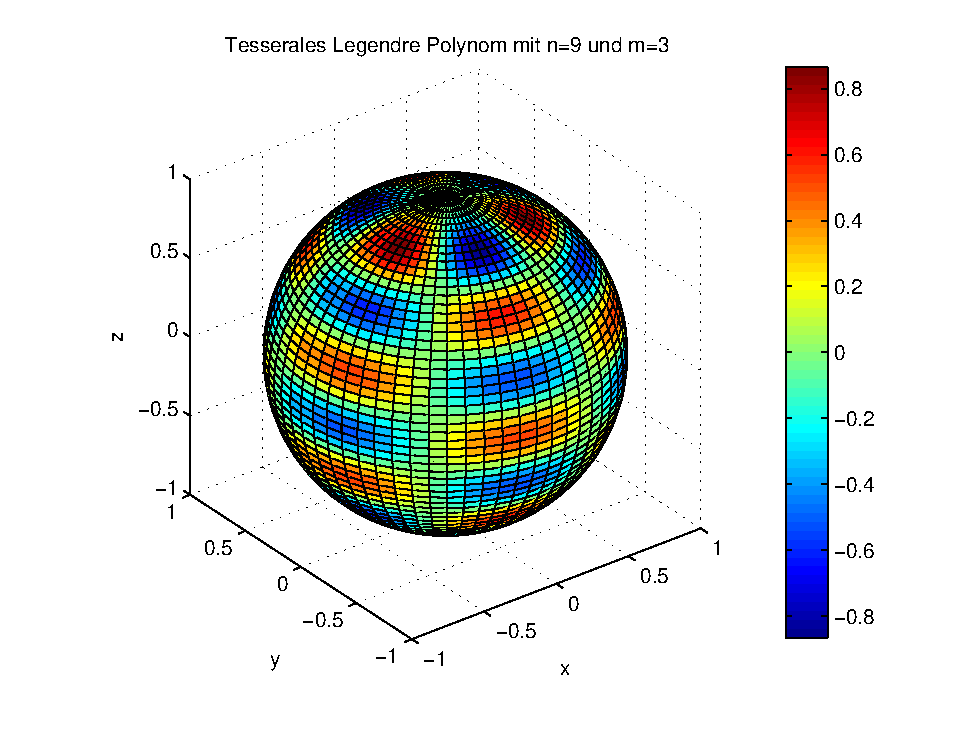
\includegraphics[scale=0.7]{tesseral.eps}
	\caption{Legendre-Polynom $P^{3}_{9}$ - tesseral}
	\end{center}
\end{figure}



\section{Aufgabenteil 2}
In dieser Aufgabe soll das Schwerefeld der Erde, welches beispielsweise aus Satellitenmessungen bekannt ist mittels der in Aufgabe 1 berechneten Legendre Polynome dargestellt werden. Die dazugeh�rigen Datens�tze zur Berechnung notwendiger Parameter haben wir der Institution des Helmholtz Centre Potsdam (GFZ German Research Centre For Geosciences) aus folgender Internetseite entnommen:\textit{http://icgem.gfz-potsdam.de/ICGEM}.\\
F�r die Aufgabenbearbeitung wurde das Datenfile \textit{osu89a.gfc} verwendet, welches die Koeffizienten der Kugelfunktionsentwicklung bis zu verschiedenen Graden und Ordnungen mit dazugeh�rigen Standardabweichungen enth�lt. Das Einlesen des Files erfolgte via load('osu.txt'). F�r die Berechnung des Potenzials ist zu beachten, dass die Koeffizienten der Polynome bis zum 10. Grad korrigiert werden (siehe Aufgabenblatt). Aufgrund der linearen Approximation des Potentials wird durch die Korrektur der Koeffizienten erreicht, dass die ersten Terme aus der Reihenentwicklung eine st�rkere Gewichtung erhalten, sodass ellipsoide Anteile (bzgl. des Referenzellipsoids) im Potentialfeld nicht �berwiegen und auch sehr geringe Anomalien zu erkennen sind. Das Programm zur Berechnung des Schwerepotentials ist folgend strukturiert:
\begin{itemize}
\item Einlesen des Datenfiles
\item Deklaration der Variablen
\item Anordnung der Koeffizienteneintr�ge in neue Matrizen $C_{nm}$ und $S_{nm}$ mit dazugeh�rigem Grad und Ordnung
\item Korrektur der Koeffizienten
\item Schleife �ber $\theta$ und $\Phi$
\item Berechnung der Legendre Polynome (+ Schmidt-Normalisierung)
\item Berechnung des Potenzials �ber Schleife (m,n) und Summenbildung
\item graphische Darstellung des Schwerepotentials
\end{itemize}
Eine detaillierte Beschreibung ist dem Programmcode im Anhang zu entnehmen.
Die Berechnung des Potenzials der Erde basiert auf folgendem Zusammenhang:
\begin{equation}
U_{g}= \frac{\gamma M}{r}\sum_{n=0}^{\infty}(\frac{a}{r})^n\sum_{m=0}^{n} P_{mn}(\theta)[C_{nm}\cos m\Phi + S_{nm}\sin m\Phi]
\end{equation}

Die zwei folgenden Abbildungen zeigen, dass variierende Ordnungen (n) der Legendre Polynome unterschiedliche Ergebnisse f�r das Schwerepotential liefern. Demnach bestimmt die H�he der Ordnungen n und damit die Anzahl berechneter Koeffizienten das Aufl�sungsverm�gen der zu ermittelnden Gr��e. Bei der Berechnung des Potentials mit n=200 werden auch kleinste Anomalien sichtbar, w�hrend f�r n=5 kleinskalige Undulationen nicht ber�cksichtigt werden. Dies ist auf die kurzwelligen Anteile der Koeffizienten zur�ckzuf�hren, welche durch eine hohe Ordnung der Kugelfl�chenfunktionen sichtbar beziehungsweise f�r Koeffizienten $n\leq 5$ unterdr�ckt werden.

\begin{figure}[h!]
	\center
	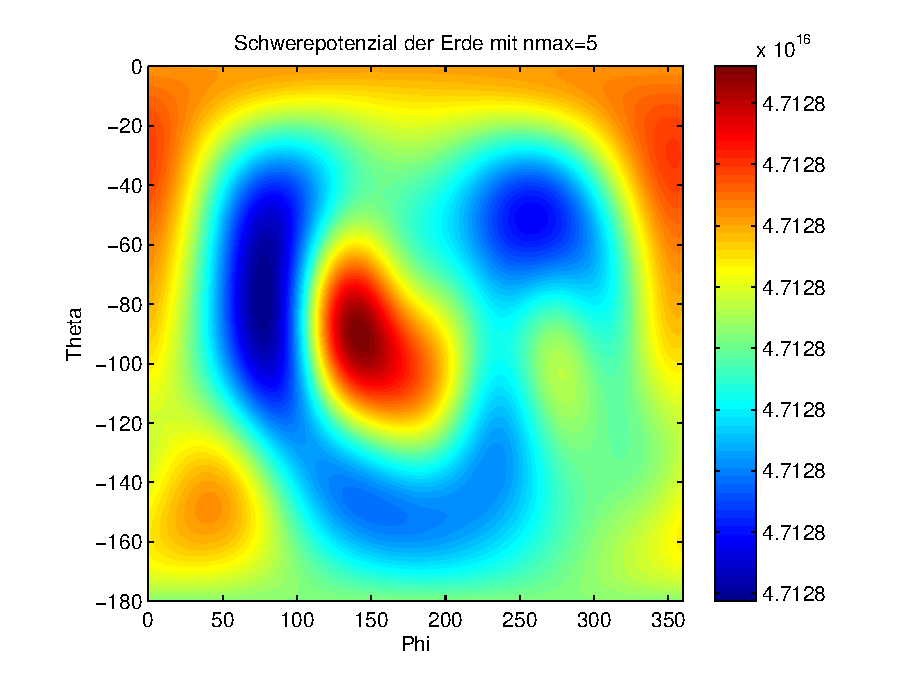
\includegraphics[scale=0.7]{nn5.eps}
	\caption{Das Schwerepotential f�r nmax=5 - sehr geringe Aufl�sung}
\end{figure}

\begin{figure}[h!]
	\center
	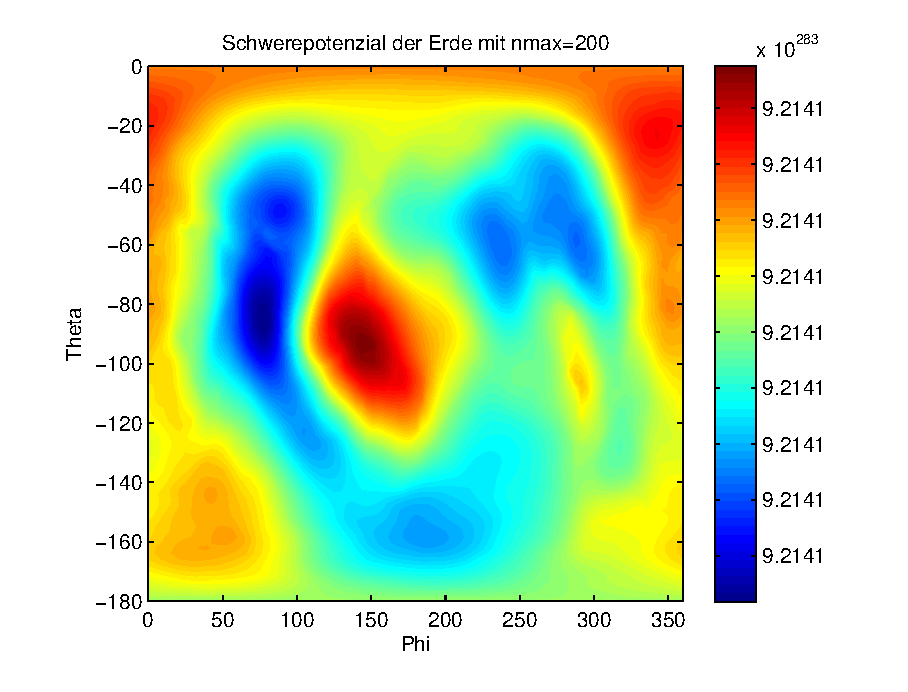
\includegraphics[scale=0.7]{nn200.eps}
	\caption{Das Schwerepotential f�r nmax=200 - geringe Anomalien sichtbar}
\end{figure}

In den anschlie�enden Abbildungen sind drei Auschnitte dargestellt die besonders starke Schwereanomalien aufweisen. Die Ursache f�r die langwelligen Anomalien sind auf gro�r�umige Dichtevariationen im Erdmantel beziehungsweise in der Erdkruste zur�ckzuf�hren. Eine h�here Gesteinsdichte erzeugt demnach eine zus�tzliche Gravitationsbeschleunigung, wodurch der Massen�berschuss eine positive Schwereanomalie bewirkt und das Geoid ''ausbeult''. Andererseits werden durch geringere Dichten negative Schwereanomalien verursacht die ''Eindellungen'' des Geoids hervorrufen. Die Dichtevariationen im Erdmantel werden durch die Geodynamik der Mantelkonvektion begr�ndet. Demnach weist extrem hei�es Mantelmaterial eine geringe Dichte auf und steigt nach oben, wogegen sich kalte Regionen durch eine hohe Dichte ausweisen und absinken. Folglich sind abtauchende Konvektionsstr�me urs�chlich f�r positive Schwereanomalien (Beulen) und aufsteigende Konvektionsstr�me verantwortlich f�r negative Anomalien (Dellen).\\
Auch die Topographie f�hrt zu lateral variablen Massenvariationen und f�hrt zu Schwereanomalien (siehe Abb.?? Himalaya)
bla bla beispiele:
\newpage
\input{aufgabe3}

%% 	APPENDIX-----------------------------------
%\begin{appendix}
\appendix
\newpage
\section{Quellcode}
\subsection{Aufgabe 1}
\lstinputlisting{Potentialtheorie_MM/Aufgabe1.m}
\newpage
\subsection{Aufgabe 2}
\lstinputlisting{Potentialtheorie_MM/Aufgabe2.m}
\newpage
\subsection{Aufgabe 3}
\subsubsection{Hauptprogramm}
\lstinputlisting{Potentialtheorie_MM/Aufgabe3.m}
\vspace{2cm}
\subsubsection{Subprogramm: Berechnen der Kreispunkte}
\lstinputlisting{Potentialtheorie_MM/kreis.m}
\vspace{2cm}
\subsubsection{Subprogramm: Berechnen der Kugel}
\lstinputlisting{Potentialtheorie_MM/kugel.m}
%\end{appendix)
\end{document}